\subsection{Caracterizaci\'on de una soluci\'on}
Una solución de nuestro problema es un subconjunto de elementos del conjunto original tal que la suma de ellos es exactamente el valor objetivo.\\
\subsection{Espacio de soluciones}
Se redefine Solución para poder hablar de factibilidad y optimalidad.\\
En la imagen podemos ver, que luego de diferentes decisiones, llegamos a diferentes soluciones (hojas) y est\'an separados en tres casos.
\begin{itemize}
	\item Los nodos rojos, verdes y celestes son las soluciones.
	\item Los nodos verdes son las soluciones factibles.
	\item Los nodos rojos son las soluciones no factibles. 
\end{itemize}	
\begin{center}
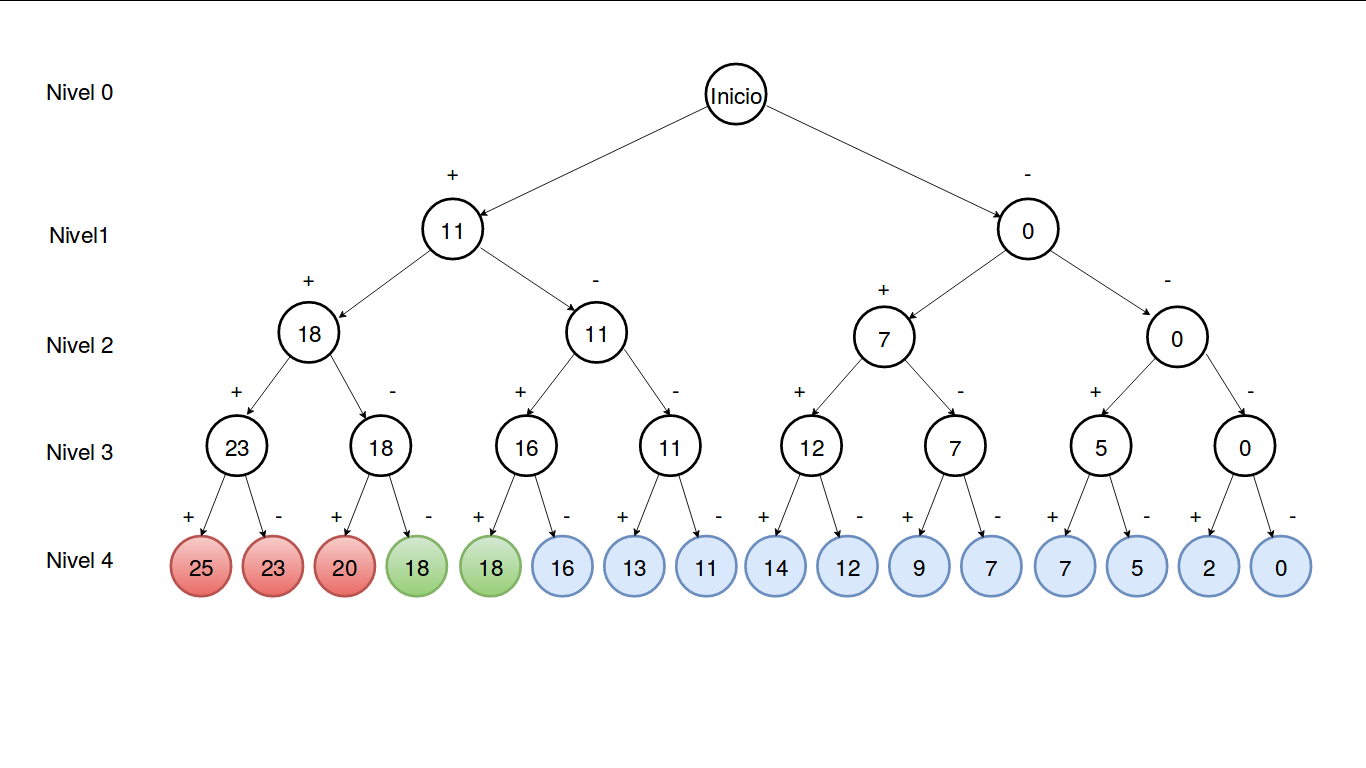
\includegraphics[width=18cm, height=10cm]{3casos.png}
\end{center}
\subsection{Recorrido del espacio de soluciones}
Se ver\'an diferentes formas de pensar el problema, y en base a ello elegiremos una forma de obtener la soluci\'on.\\

\begin{itemize}
\item La primer forma de ver el problema es simple, mirar todo el espacio de soluciones y quedarnos con la mejor.\\
\item En la segunda forma trataremos de recorrer solamente el espacio de soluciones factibles.\\
\item La tercer forma va mas enfocado a cuando una soluci\'on es mejor que otra, y veremos como recorrer las soluciones que son mejores que la soluci\'on que tenemos hasta el momento (si las hay, sino podaremos).\\
\item La \'ultima forma de pensar el problema sera ver los problemas anteriores inmediatos y ver como con ellos se puede construir el problema mas grande.
\end{itemize}